\documentclass{article}
\usepackage[utf8]{inputenc}
\usepackage{graphicx}
\usepackage{minted}
\usepackage[demo]{graphicx} % Required for including images
\usepackage[font=small,labelfont=bf]{caption}
\graphicspath{ {images/} }
\makeatletter
\renewcommand\tableofcontents{%
    \@starttoc{toc}%
}
\makeatother

\title{\huge{Edit Distance}\\{with or without n-gram ?}}
\author{Vivoli Emanuele}
\date{Giugno 2017}

\begin{document}

\maketitle
\vspace*{0.30\textheight}
\tableofcontents

\newpage
\section{Introduzione}
Lo scopo dell'esercizio è trovare all'interno di un lessico la parola più vicina alla parola data (o una lista di parole vicine). La definizione di vicinanza verrà data nella sezione interessata ( "Teoria" ), ma indicativamente si definisce parola a distanza minima quella che è piu simile alla parola data a meno di errori di digitazione (quindi invertendo delle lettere, o tralasciandone alcune).   
E' necessario utilizzare allo scopo dell'esercizio la funzione di Edit Distance vista a lezione, ma analizzare anche le differenze tra l'uso e il non uso degli n-gram all'interno della ricerca.
Dovremmo dunque trovare una serie di test sul lessico, e successivamente sui file n-gram precedentemente creati, che può essere un buon punto di partenza per analizzare e confrontare le velocità di esecuzione della ricerca con o senza successo della parola a distanza minima.
Per avere maggior tangibilità della differenza fra queste due implementazioni della risoluzione del problema, si decide di mostrate mediante grafici e tabelle i risultati sperimentali dell'esercizio, testando la ricerca su lessici formati da 9000, 60000, 280000 parole.

I test che verranno svoti sui lessici saranno approfonditi successivamente nella sezione "Descrizione Esperimenti", ma proviamo a dare una vista indicativa su ciò che faremo nel programma:
verranno scelte delle parole randomicamente all'interno di ogni lessico, e cercata la parola a distanza minima sia nei file n-gram precedentemente creati, sia all'interno del lessico stesso. Verranno successivamente effettuate delle modifiche alla parola, cambiando uno o piu caratteri, randomizzando tutti i caratteri della parola, aggiungendone uno o levandolo; in modo da avere piu test su una parola, e simulando gli errori di digitazione reali che spesso vengono erroneamente fatti dalle persone digitando velocemente o distrattamente.

\newpage
\section{La Teoria}
\subsection{Distanza di Editing}
Per trasformare una stringa di input $x[1...m]$ in una stringa di output $y[1...n]$, possiamo svolgere varie operazioni. Date le stringhe $x$ e $y$ il nostro obiettivo è effettuare una serie di trasformazioni che cambiano $x$ in $y$. Ci sono cinque operazioni di trasformazione alle quali attribuiamo un costo in base a come possono presentarsi:
\begin{description}
\item [Copia] di un carattere, il costo è $0$ poiche si tratta di lasciare immutato l'elemento in $x$ e andare a visitare gli elementi successivi di entrambe le stringhe.
\item [Sostituzione] di un carattere con un altro, costo $1$ poiche corrisponde a sovrascrivere un carattere in $x$ con quello rispettivo in $y$, e visitare i successivi caratteri di entrambi.
\item [Cancellazione] di un carattere in $x$, costo $1$, e proseguire con l'analisi nel resto della stringa.
\item [Inserimento] di un carattere in $x$, anche qui costo $1$ e proseguo in entrambe le stringhe.
\item [Scambio] fra due caratteri adiacenti in $x$, costo $1$ poiche spesso produciamo questo errore nel digitare delle parole, e poiche non avrebbe senso valutarlo come una combinazione di cancellazione, copia e inserimento (totale costo $2$) in quanto non sarebbe mai valutato nella sequenza di operazioni a causa del controllo fra il costo minore, che vedremo nella sezione di "Documentazione"; si prosegue poi con gli elementi di due posizioni successive.
\end{description}
Segue la definizione di \textbf{Distanza di Editing} alla quale alludevamo nell'introduzione:

Date due sequenze $x[1...m]$ e $y[1...n]$ e un insieme di costi di trasformazione, la \textbf{Distanza di Editing} tra $x$ e $y$ è il costo della sequenza di operazioni più economica che trasforma $x$ in $y$. 

Poiche l'Algoritmo di Edit Distance appartiene al campo della Programmazione Dinamica, i passi che esso svolge per procedere alla costruzione della soluzione ottima del problema richiesto partono dal calcolare la soluzione ottima in metodologia "bottom-up", partendo dai sottoproblemi più semplici fino a queli sempre più complessi, e poi al problema principale.

L'utilizzo dell'algoritmo Edit Distance nella correzione ortografica riguarda i campi più svariati, a partire dal suo impiego nella correzione di parole scritte in modo errato all'interno di documenti, fino a suggerire le query all'utente che desidera cercare qualcosa nel web.

\subsection{Distanza di Editing Pesata}
Corrisponde alla Edit Distance che abbiamo poco sopra introdotto, dove però il costo di un operazione dipende dai caratteri coinvolti e non solo dal tipo di operazione.
(es. $o$ confuso più spesso con $i$ che con $s$,sostituendo $o$ con $i$ dovrei avere Edit Distance inferiore)
Serve, per poter implementare questa funzione, una "matrice dei pesi" che dipende dall'applicazione.

\textbf{Piccola parentesi inerente ai test:} Nel nostro caso è un po' troppo positivo paragonare la logica di scambio di caratteri vicini della tastiera con la vera implementazione di tale "pesatura" svolta dalla Distanza di Editing Pesata, ma ciò che si tenta di fare è una semplicizzazione di questa implementazione più corposa ed esaustiva.

\subsection{Intersezione di n-gram}
Se un compito assegnato fosse quello di trovare, dato un lessico L e una stringa Q, all'interno di L le parole più vicine a Q, quali alternative avremmo? 

Potrei confontare Q con tutte le parole di L, e selezionare quella con Distanza di Editing minore, ma sembra troppo costoso anche solo a pensarci. 
Potrei elencare a partire da Q tutte le parole con Edit Distance minore di una certa soglia (ad es. 2) e intersecare tale insieme con il Lessico L per vedere se ne esiste una a distanza minore, ma anche qui genererei delle parole che non esistono all'interno del lessico, spendendo molto tempo per scorrere il Lessico e confrontare tali parole con ognuna fino a scoprire che non appartengono all'insieme interserzione. 
Potrei quindi pensare ad un modo per ridurre l'insieme dei termini candidati all'interno del Lessico: \textbf{Intersezione di n-gram}.
Data la parola Q da cercare all'interno di L, divido in n-gram la parola Q con n scelto precedentemente (dall'analisi seguirà che un valore buono per la scelta di n è 3), e cerco per ogni parola di L se possiede un numero considerevole di n-gram comuni a quelli di Q in base ad un coefficente chiamato Coefficente di Jaccard (quoziente tra la dimensione dell'insieme intersezione e quella dell'insieme unione). Su questo insieme di parole posso quindi calcolare l'Edit Distance e selezionare la parola più vicina.

es. 3-gram
\begin{description}
\item[L = november]; 3-gram: nov, ove, vem, emb, mbe, ber
\item[Q = december]; 3-gram: dec, ece, cem, emb, mbe, ber
\item[JC:] $3/9 = 0.3$
\end{description}
Per trovare i termini considero una soglia $JC > 0.8$

\section{Aspettative}
Prima di studiare i risultati pratici che l'esecuzione del programma ci potrà mostrare, possiamo già fare un'analisi riguardo al comportamento che ci aspettiamo.

La prima considerazione necessaria da fare riguarda proprio la differenza di implementazione dell'esercizio utilizzando o meno la tecnica "indici n-gram".
Infatti per la decomposizione in n-gram viene fatto partire, separatamente dai test, un programma che si occupa di scomporre ogni parola in n-gram (con $n$ appartenente a [1, 2, 3, 4]) e salvare tale parola all'interno di un file denominato con la medesima sigla del gram. In questo modo si avrà per ogni Lessico una cartella contenente a sua volta 4 cartelle, una per ogni dimensione del gram, e a loro volta all'interno di ogni cartella tanti file quanti sono i gram diversi che si sono incontrati nella decomposizione.
E' necessario fare una precisazione riguardo a quello che succedera nella decomposizione, poichè con indice di n-gram via via crescente saranno sempre meno le parole all'interno dei file, ma sempre più file diversi fino a $n$ uguale a $4$ dove si hanno circa $25000$ file diversi. (Dalla teoria delle probabilità segue che il numero massimo di file n-gram al variare di $n$ è dunque $k^n$, con $k$ caratteri dell'alfabeto in utilizzo, ed $n$ indice dei gram). 
Si ha quindi che l'utilizzo degli n-gram comporta un tempo aggiuntivo di decomposizione al quale non possiamo sottrarci e che dobbiamo fortemente considerare poichè puo essere causa di corposi rallentamenti del sistema (dipende dalla velocità di calcolo della macchina, ma il tempo di decomposizione varia da 1 ora e mezzo fino a 6 ore, per un lessico di 230000 parole).


Riguardo ai test che svolgeremo si fanno delle predizioni basate più sull'intuito che sulla teoria poichè la logica ci suggerisce un confornto fra i tempi di esecuzione dei due tipi di implementazione differenti: per l'implementazione diretta sul lessico, bypassando la decomposizione in n-gram, si ha che dobbiamo calcolare per ogni parola del Lessico l'edit discance ed aggiungere la tupla [parola : val] alla lista dei minori, e aggiornare il minimo se necessario. Il costo potrebbe essere un $\O{len(parola più lunga)*m*len(L)}$ dividendolo nel costo del calcolo dell'Edit Distance che è quadratico (in realtà $\theta{n*m}$ ma considerando la lunghezza della parola più lunga del Lessico si ha $\0{len(parola più lunga)*m}$ ), ed il costo per scorrere il Lessico $\theta{len(L)}$.
Il costo di esecuzione aspettato utilizzando gli n-gram è invece di gran lunga inferiore (dipende in realtà dall'indice $n$ che adottiamo) poichè ogni parola che non ha n-gram in comune con quelli della parola Q data, non è presente in nessun file di quelli che visiteremo. Ogni file ha al suo interno tutte le parole che contengono quel n-gram, e su ogni parole di ogni file interessato viene calcolato il coefficente di Jaccard indicato con CJ e solo se soddisfa i requisiti ($CJ > 0.6$) calcolato l'Edit Distance. Nonostante si abbia la certezza che una parola "molto vicina" a Q appartenga a più di un file interessato, e dunque venga più volte controllato il CJ e calcolato l'Edit Distance, si ipotizza a rigor di logica che il costo sia di gran lunga inferiore rispetto a calcolare su ogni parole del Lessico la distanza di Editing, e vedremo dagli esperimenti pratici se questa ipotesi viene confermata o meno.

\newpage

\section{Descrizione esperimenti}
L'esperimento condotto ha lo scopo di capire quale sia l'andamento dei tempi di ricerca della parola più vicina all'interno di un lessico L ad una certa parola Q data, utilizzando o meno la logica della decomposizione in n-gram, ed in aggiunta il coefficente di Jaccard per verificare se tale parola di n-gram è candidata ad essere la migliore oppure no.
Testare dunque i due casi saranno i nostri esperimenti.
Per ogni lessico L si scelgono 5 parole randomicamente e si testano 6 modifiche di queste parole per ogni n-gram scelto (considerando $n = 0$ il non utilizzo degli n-gram).
I test che vengno fatti si trovano dunque all'interno di cicli annidati nel file $"test.py"$ come vedremo.

\subsection{Codice di calcolo}
\inputminted{python}{python.py}
La classe test non contiene una vera e propria funzione main(), ma una serie di istruzioni che caratterizzano il ciclo principale che scorre i vari file confrontando ed inserendo i valori trovati all'interno di una matrice di più indici. Ogni ciclo interno ha il proprio ruolo che, come possiamo vedere dal codice, opera nel seguente modo:
\begin{itemize}
    \item Un ciclo che scorre la lista dei lessici che vogliamo testare.
    \item Un ciclo che scorre le 5 parole prelevate randomicamente dal lessico. 
    \item Un ciclo che scorre gli indici $n$ degli n-gram e testa le 6 modifiche sulla parola calcolando tempi di esecuzione, parola e distanza minima, e coefficente di Jaccard.
\end{itemize}
Possiamo vedere come le modifiche sulla parola data siano rispettivamente:
\begin{description}
    \item[1] Parola Q con nessuna modifica, si cerca dunque al parola stessa all'interno del lessico (utilizzando o meno gli n-gram)
    \item[2] Parola Q con ogni carattere cambiato di posto (randomicamente)
    \item[3] Parola Q senza un elemento in posizione random
    \item[4] Parola Q con l'aggiunta di un elemeto random in posizione random
    \item[5] Parola Q con un elemento cambiato con uno dei vicini (nella tastiera QWERTY)
    \item[6] Parola Q con due elementi cambiati con uno dei vicini (nella tastiera QWERTY)
\end{description}

\newpage
\section{Documentazione}
Per l’esercizio sono utilizzati tre programmi che hanno i seguenti macro-ruoli:
\begin{itemize}
\item Un programa (editDistance.py) che contiene le seguenti funizoni:
\begin{description}
\item[edit\_distance(x, y)]: funzione che dati $x$ e $y$ ne calcola l'edit distance, basandosi sui costi dettati dalla funzione cost()
\item[cost(operator)]: che stabilisce il costo di un operazione, data in input la stringa che definisce l'operazione svolta, ritorna il costo
\item[n\_gram\_decompose(x, n)]: dato $x$ la parola e n l'indice di gram, ritorna la lista degli n-gram che sono contenuti in $x$
\item[jaccard(x\_gram, y\_gram)]: calcola il coefficente di Jaccard per le parole $x$ e $y$ che gli vengono passate
\item[n\_gram\_compare(path, x, n)]: se $n = 0$ siamo nel caso in cui non si deve usare la logica n\-gram, e si richiama la funzione $all_compare(path, x)$, altrimenti si scorrono tutti i file che si chiamano con il nome degli n-gram contenuti nella parola $x$ da cercare, e si calcola il coefficente di Jaccard su ogni riga dei file, se sono dei candidati si calcola l'Edit Distance ed eventualmente si aggiorna la parola a distanza minima
\item[all\_compare(path, x)]: scorre tutte le righe del file Lessico, e per ogni riga calcola l'Edit Distace con $x$ ed eventualmente aggiorna la parola a distanza minima
\item[file\_to\_gram(path, n\_gram)]: viene eseguito solamente una volta per ogni Lessico e decompone il lessico in n\-gram, con $n$ in [1, 2, 3, 4]. 
\end{description}

\item Un programma (test.py) che esegue i test che abbiamo descritto nella sezione precedente "Codice di Calcolo", e che memorizza al termine i risultati (salvati teporaneamente su di una lista di liste indicizzata come una matrice a 5 dimensioni) su di un file pickle, in modo da poter riusare i dati utilizzati precedentemente per visualizzarli, studiarli e farne le considerazioni necessarie senza dover ogni volta ricompilare il codice (operazione di gran lunga dispendiosa).

\item Un programma (exp.py) che decompone i pickle salvati nel programma "test.py" negli oggetti originali, e elabora i risultati numerici sottoforma di grafici (che verranno ampliamente esaminati successivamente).
\end{itemize}
 

\newpage
\section{Risultati Sprimentali}

\subsection{Distanza minima}

\begin{center}
\begin{minipage}{0.8\linewidth}


    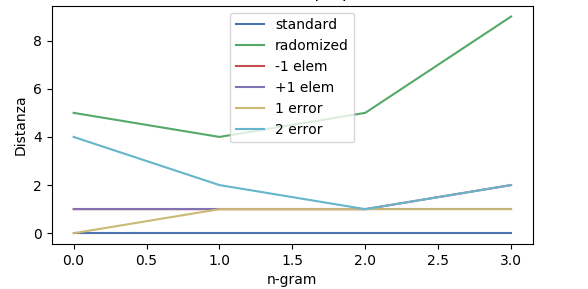
\includegraphics[width=\linewidth]{img/dist_9K.png}
    \captionof{figure}{9000 parole}
\end{minipage}%
\hfill
\begin{minipage}{0.8\linewidth}
    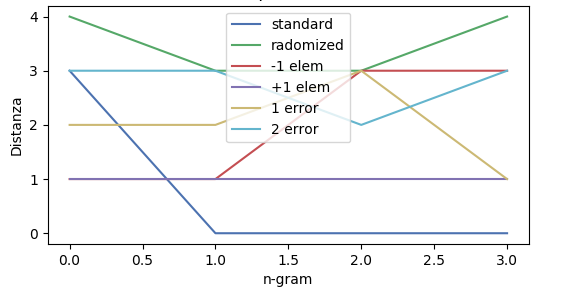
\includegraphics[width=\linewidth]{img/dist_60K.png}
    \captionof{figure}{60000 parole}
\end{minipage}%
\hfill
\begin{minipage}{0.8\linewidth}
    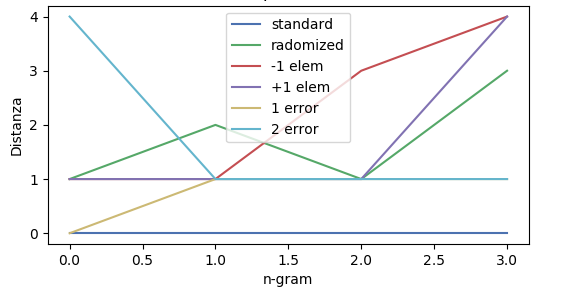
\includegraphics[width=\linewidth]{img/dist_280K.png}
    \captionof{figure}{280000 parole}
\end{minipage}% 
\end{center}

I primi risultati sperimentali ci mostrano che modificando una parola Q si può presentare, con un errore variabile, un insieme di parole $P_i$ in L che in base alla valutazione del coefficente di Jaccard, sono o meno candidate ad essere le parole a distanza minima da Q. Questo sta a significare che il coefficente di Jaccard è un forte limite per la decisione delle parole candidate (poichè istituisce una costante di "gusto" che nel caso venisse meno, la parola è considerata non candidata e non ne viene calcolato l'Edit Distance). 
Si presenta con tale implementazione del Coefficente di Jaccard, e dell'Edit Distance a seguire, che il valore di JC e della distanza minima va interpretato almeno con un esempio per poterne capire le potenzialità, i pregi e i difetti.
Proviamo a considerare il caso "1 error" ( nel qual caso viene scelto un carattere all'interno della parola e viene cambiato con uno adiacente nella tastiera qwerty, in modo da simulare un errore di digitazione di un essere umano) e lasciare al lettore l'analisi dei restanti casi, analizzando il caso della modifica di un crattere della parola Q:"arcobaleno" ottenendo $Q_1$:"arcoboleno".
Per ogni indice $n$ valutiamo gli n-gram della parola $Q_1$ e della rispettiva parola Q che sto cercando, in modo da vedere quanto puo essere selettivo il JC.
\begin{description}
\item[indice n=2]:

$Q_1$ = [ar, rc, co, ob, bo, ol, le, en, no]

Q  = [ar, rc, co, ob, ba, al, le, en, no]

${\|$Q$\cap$Q_1$\|}\div{\|$Q$\cup$Q_1$\|}$ = 0.63; si ha dunque che al variare di un carattere all'interno della parola vengono cambiati due 2-gram, e dunque non si controllerà più all'interno di quei file. La parola cercata si presenterà comunque negli altri file più volte, e quando si confronta tale parola Q con quella che stiamo cercando $Q_1$ viene calcolato un JC $0.63>0.5$ che abbiamo impostato come limite, quindi per $n=2$ possiamo essere soddisfatti del nostro metodo.

\item[indice n=3]: 

$Q_1$ = [arc, rco, cob, obo, bol, ole, len, eno]

Q  = [arc, rco, cob, oba, bal, ale, len, eno]

${\|$Q$\cap$Q_1$\|}\div{\|$Q$\cup$Q_1$\|}$ = 0.4;
si ha dunque che al variare di un carattere all'interno della parola vengono cambiati tre 3-gram, e dunque non si controllerà più all'interno di quei file. La parola cercata si presenterà comunque negli altri file più volte, ma quando si confronta tale parola Q con quella che stiamo cercando $Q_1$ viene calcolato un JC $0.4<0.5$ che abbiamo impostato come limite, e si comprende adesso il problema dell'utilizzo di tale "coefficente di gusto". Se invece viene cercata una parola $Q_2$:"arcobalena" si ha che varia solamente un indice 3-gram (l'ultimo), di questa parola viene quindi calcolata la distanza ottenendo un edit Distance = 1. Stesso valore della precedente $Q_1$, che pero' è stata scartata.
Questa tecnica è non ottimale, ed una semplice modifica del valore JC da $0.5$ a $0.4$ potrebbe includere delle soluzioni che prima non consideravamo.

\item[indice n=4]: 

$Q_1$ = [arco, rcob, cobo, obol, bole, olen, leno]

Q  = [arco, rcob, coba, obal, bale, alen, leno]

${\|$Q$\cap$Q_1$\|}\div{\|$Q$\cup$Q_1$\|}$ = 0.27;
si ha dunque che al variare di un carattere all'interno della parola vengono cambiati quattro 4-gram, e dunque non si controllerà più all'interno di quei file. La parola cercata si presenterà comunque negli altri file più volte, ma quando si confronta tale parola Q con quella che stiamo cercando $Q_1$ viene calcolato un JC $0.27 < 0.5$ che abbiamo impostato come limite. Potremmo proporre almeno due differenti soluzioni: una come la precedente, di abbassare la soglia imposta dal JC in modo che se viene variato un carattere nella parte centrale della parola, anche se la maggior parte dei 4-gram non coincidono, se ne calcola lo stesso l'Edit Distance. Si può inoltre ampliare questa condizione calcolando di fatto la distanza fra i 4-gram che non coincidono, in modo da evitare che la parte centrale sia totalmente diversa, e non per solo un carattere, potendo fare quindi una selezione fra le parole a basso JC ma che però sono buone candidate, e le parole a basso JC che non hanno nulla a che fare con l'esser vicini alla parola Q cercata. Potrebbe quest'ultima soluzione essere molto costosa e convenire semplicemente l'impostazione più bassa del JC e il calcolo della distanza direttamente sulla parola, piuttosto che molteplici volte sui 4-gram. 
\end{description}

\subsection{Tempo di esecuzione}

\begin{center}
\begin{minipage}{0.8\linewidth}
    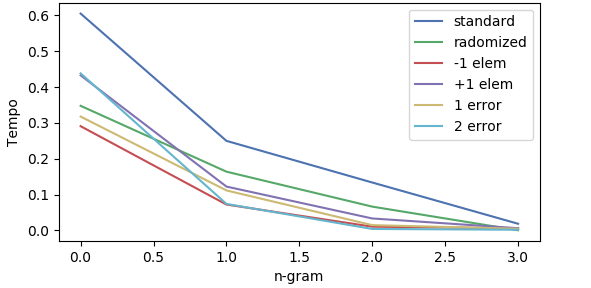
\includegraphics[width=\linewidth]{img/time_9K.png}
    \captionof{figure}{9000 parole}
\end{minipage}%
\hfill
\begin{minipage}{0.8\linewidth}
    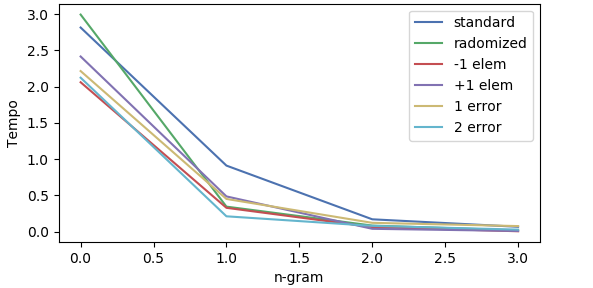
\includegraphics[width=\linewidth]{img/time_60K.png}
    \captionof{figure}{60000 parole}
\end{minipage}%
\hfill
\begin{minipage}{0.8\linewidth}
    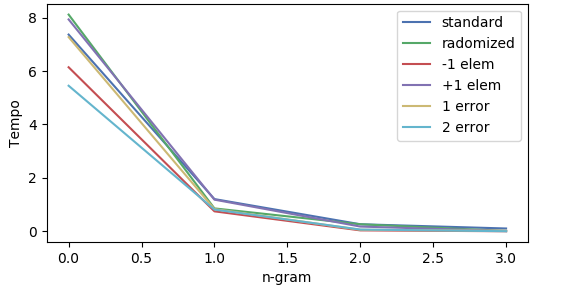
\includegraphics[width=\linewidth]{img/time_280K.png}
    \captionof{figure}{280000 parole}
\end{minipage}% 
\end{center}


\begin{table}[htbp]
\centering 
\caption{\textbf{9K} calcolo Tempi di esecuzione (media)}
\begin{tabular}{l c c c c c}
\hline\hline
\multicolumn{1}{c}{\textbf{Test}}& \textbf{senza n-gram}& \textbf{1-gram} & \textbf{2-gram}& \textbf{3-gram}\\ \hline
Standard    & 2.814 & 0.910 & 0.170 & 0.067\\
Randomized  & 2.993 & 0.345 & 0.083 & 0.017\\
-1 element  & 2.060 & 0.328 & 0.063 & 0.006\\
+1 element  & 2.415 & 0.485 & 0.039 & 0.009\\
1 qwerty err & 2.214 & 0.451 & 0.121 & 0.076\\
2 qwerty err  & 2.123 & 0.211 &  0.079 & 0.028\\
\hline
\end{tabular}

\caption{\textbf{60K} calcolo Tempi di esecuzione (media)}
\begin{tabular}{l c c c c c}
\hline\hline
\multicolumn{1}{c}{\textbf{Test}}& \textbf{senza n-gram}& \textbf{1-gram} & \textbf{2-gram}& \textbf{3-gram}\\ \hline
Standard    & 2.814 & 0.910 & 0.170 & 0.067\\
Randomized  & 2.993 & 0.345 & 0.083 & 0.017\\
-1 element  & 2.060 & 0.328 & 0.063 & 0.005\\
+1 element  & 2.415 & 0.486 & 0.039 & 0.009\\
1 qwerty err & 2.214 & 0.451 & 0.122 & 0.076\\
2 qwerty err & 2.123 & 0.211 & 0.079 & 0.028\\
\hline
\end{tabular}

\caption{\textbf{280K} calcolo Tempi di esecuzione (media)}
\begin{tabular}{l c c c c c}
\hline\hline
\multicolumn{1}{c}{\textbf{Test}}& \textbf{senza n-gram}& \textbf{1-gram} & \textbf{2-gram}& \textbf{3-gram}\\ \hline
Standard    &  7.368 & 1.205 & 0.262 & 0.103\\
Randomized  &  8.117 & 0.856 & 0.262 & 0.010\\
-1 element  &  6.143 & 0.746 & 0.033 & 0.001\\
+1 element  &  7.935 & 1.184 & 0.176 & 0.009\\
1 qwerty err &  7.273 & 0.831 & 0.055 & 0.016\\
2 qwerty err &  5.451 & 0.812 & 0.064 & 0.002\\
\hline
\end{tabular}

\end{table}

Possiamo vedere da questi grafici come le aspettative che avevamo sull'andamento temporale del calcolo della minima distanza si sono verificate sperimentalmente, e come si ha una conferma netta del minor tempo di esecuzione per il caso di utilizzo di n-gram, piuttosto che l'Edit Distance su ogni elemento del Lessico. Dovremmo fare un ulteriore analisi differenziando i valori trovati al variare di n nell'utilizzo degli indici n-gram poichè all'aumentare di n il tempo di esecuzione, se pur non così considerevolmente, cala quasi linearmente. 
Questo fenomeno è giustificato dal fatto che, nonostante faccia il calcolo dell'Edit Distance solo nel caso in cui il coefficente $JC>0.6$, i file n-gram crescono di dimensione via via che diminuisce l'indice n. Dunque il tempo di esecuzione della ricerca del minimo per ogni test con n-gram sarà piu' grande all'indice 1, e poi via via decrescendo in 2 e 3.

\textbf{NB}: nonostante si sia consapevoli che non ha senso utilizzare un indice n-gram troppo basso (come $1$) o tropo alto (come $4$) se le parole del lessico sono non più lunghe di 9 caratteri al massimo, si utilizza l'indice $1$ al solo fine di mostrare come variano il tempo e la Distanza minima all'aumentare o al diminuire di n.

\subsection{Coefficente Jaccard}

\begin{center}
\begin{minipage}{0.48\linewidth}
    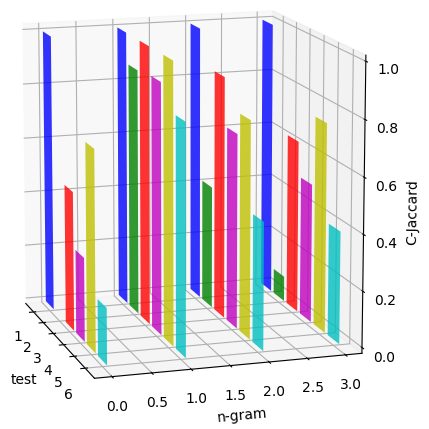
\includegraphics[width=\linewidth]{img/jc_9K.png}
    \captionof{figure}{9000 parole}
\end{minipage}%
\hfill
\begin{minipage}{0.48\linewidth}
    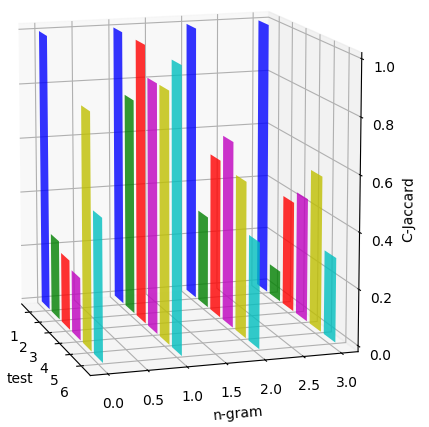
\includegraphics[width=\linewidth]{img/jc_60K.png}
    \captionof{figure}{60000 parole}
\end{minipage}%
\hfill
\begin{minipage}{0.48\linewidth}
    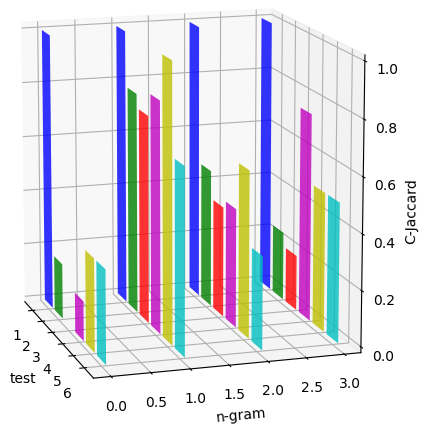
\includegraphics[width=\linewidth]{img/jc_280K.png}
    \captionof{figure}{280000 parole}
\end{minipage}% 
\captionof{figure}{Coefficente di Jaccard per test ed n-gram}
\end{center}

Si è voluto inoltre "plottare" il coefficente di Jaccard delle parole che sono state selezionate come \textbf{parole a distanza minima} da $Q$ cercata.

\end {document}



%   Viene adesso elencata in modalità "lista dela spesa" la sequenza di test che viene svolta, in modo     da facilitare la chematizzazione della stessa per comprenderne meglio lo scopo:
%   (per ogni lessico si procede allo stesso modo, e dunque:)
%   -   si scelgono n parole randomicamente all'interno del lessico
%       (per ogni parola si procede allo stesso modo, e dunque:)
%       -   per ogni dimensione n-gram [1, 2, 3, 4]
%           -   si divide la parola in n-gram e si cerca all'interno dei file che si chiamano con il nome      del n-gram la parola con distanza minima e si salva la parola, la distanza, il tempo di        esecuzione della ricerca, il coefficente di Jaccard (che introdurremo in "Teoria").
%        -   si randomizza la parola data in base alle lettere e si cerca all'interno dei file che si       chiamano con il nome del n-gram la parola con distanza minima e si salvano i soliti dati.
%        -   si leva un carattere dalla parola data e si cerca all'interno dei file che si chiamano con     il nome del n-gram la parola con distanza minima e si salvano i soliti dati.
%        -   si aggiunge un carattere dalla parola data e si cerca all'interno dei file che si chiamano     con il nome del n-gram la parola con distanza minima e si salvano i soliti dati.
%        -   si scambia uno dei caratteri che solitamente viene scambiato, con un suo vicino nella          tastiera qwerty, come "i con o" o viceversa, (simulando dunque un weighted edit distance) e si cerca all'interno dei file che si chiamano     con il nome del n-gram la parola con distanza minima e si salvano i soliti dati.
%        -   si scambiano due dei caratteri che solitamente vengono scambiati, con un loro vicino nella     tastiera wasd, come "i con o" o viceversa, e si cerca all'interno dei file che si chiamano     con il nome del n-gram la parola con distanza minima e si salvano i soliti dati.